\paragraph{Signatures including a Z boson}

\subparagraph{Z+\MET signature, leptonic channel}

\begin{table}
\centering
\caption{Event selection requirements for the analysis of the Mono-Z signature with leptonic Z decays.
        The requirements are inspired to follow those used in typical experimental analyses.}
\begin{tabular}{c | c |r l}
Selection stage & Quantity & Requirement \\\hline


\multirow{ 2}{*}{Inclusive}         & lepton $\left|\eta\right|$                    & $< 2.5$ \\
                                    & leading (trailing) lepton \pt                 & $> 25 (20)$ GeV \\\hline

\multirow{ 2}{*}{Preselection}      & $\left|m_{ll}-m_{Z,\mathrm{nominal}}\right|$  & $< 15$ GeV\\
                                    & \MET                                          & $> 40$ GeV \\\hline

\multirow{ 3}{*}{Final selection}   & $\Delta\Phi(ll,\MET)$                         & $>2.7$\\
                                    &$|p_{T,ll} - \MET|/p_{T,ll}$                   & $<0.4$\\
                                    &  $\Delta R(ll)$                               & $<1.8$\\
                                    &  \MET                                         & $>80$ GeV \\ 
\end{tabular}


\label{tab:monozll_selection}

\end{table}

Inclusive distributions of the invariant masses of the dilepton and $\chi\chi$ systems are shown in \autoref{fig:monoz_kin_inclusive} (before preselection). Independently of the parameters, the dilepton mass spectrum is centered at the Z peak, without any nonresonant contribution. The $M_{\chi\chi}$ distribution illustrates the signal contributions from different diagrams. For $\mA>\ma$, DM is dominantly produced from on-shell $a$ boson production. In the inverted mass region $\mA<\ma$, the situation is reversed, and $H$ diagrams dominate.

\begin{figure}
\centering
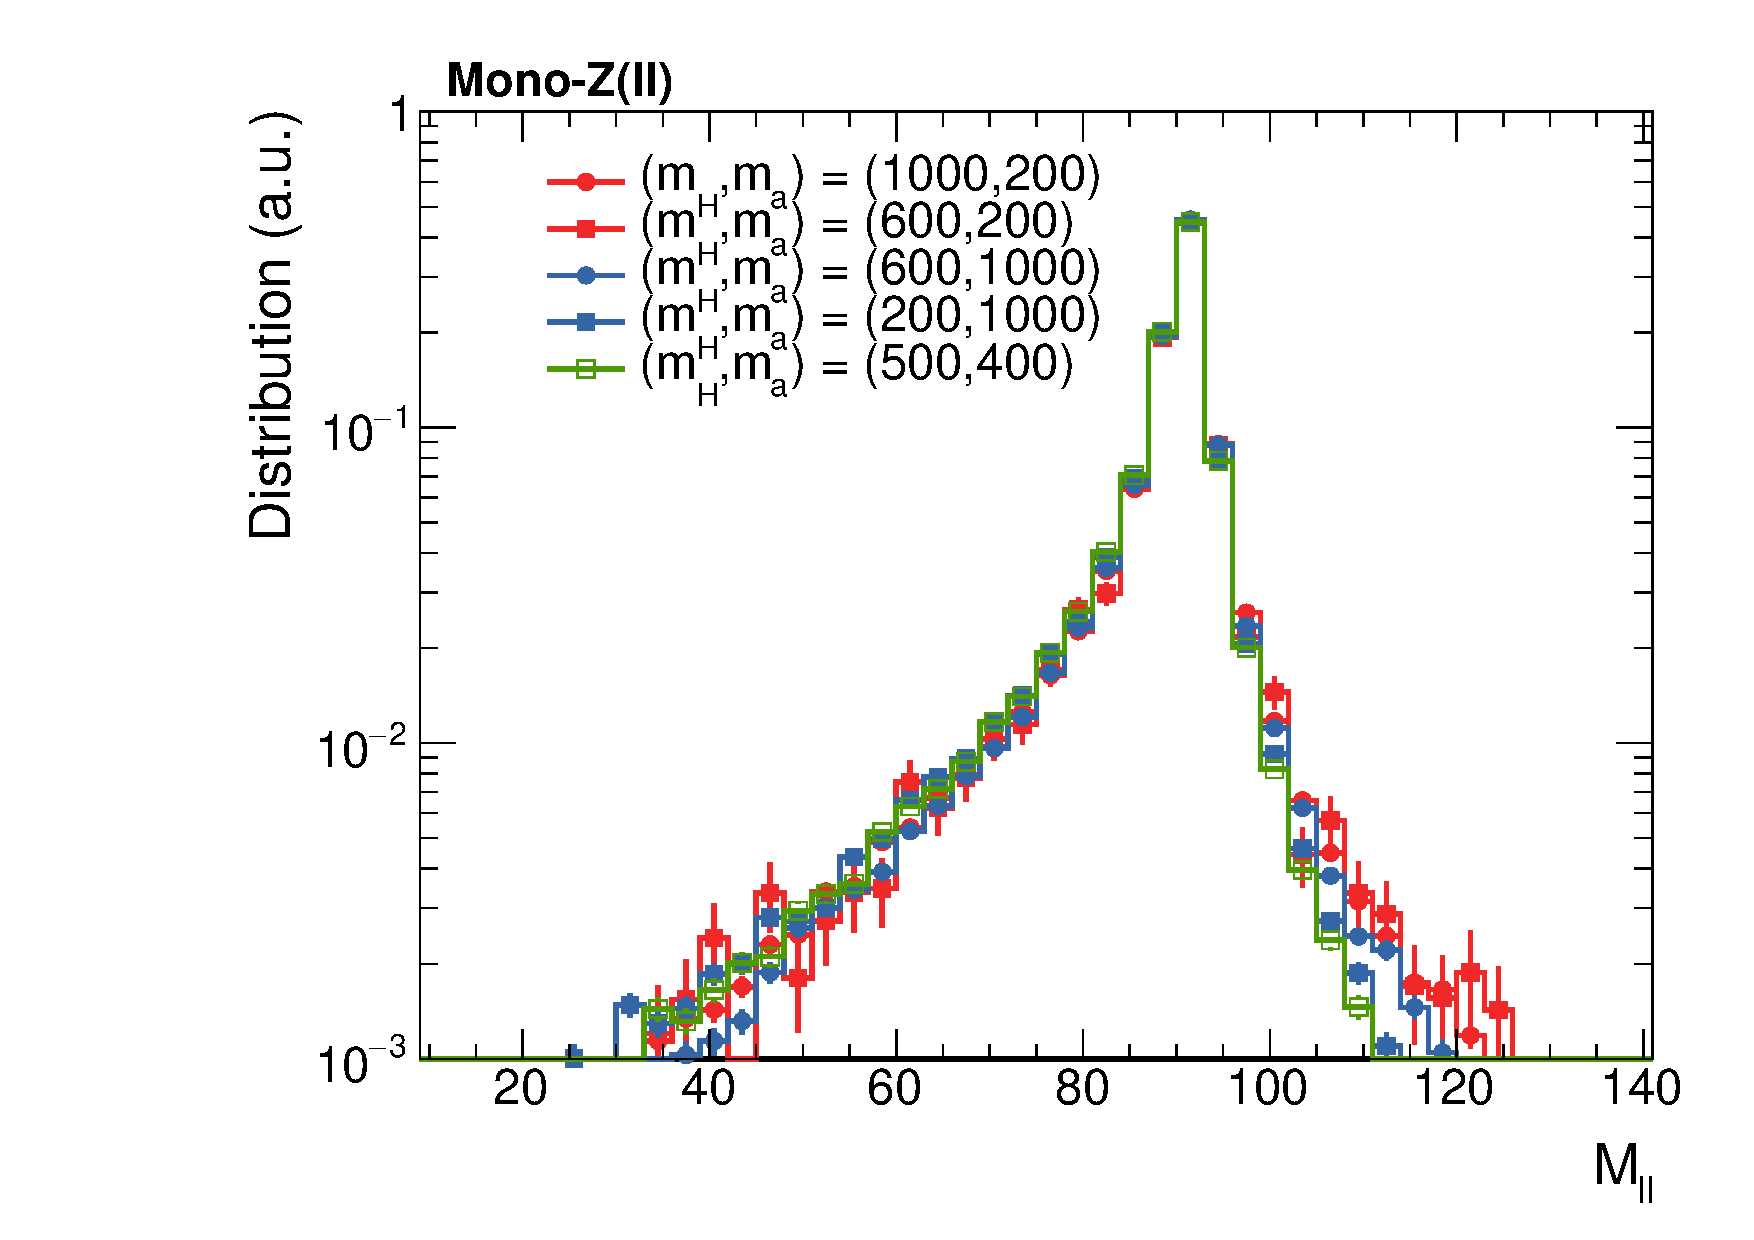
\includegraphics[width=0.45\textwidth]{texinputs/04_grid/figures/monoz/leptonic/inclusive_h_mz_lep.pdf}
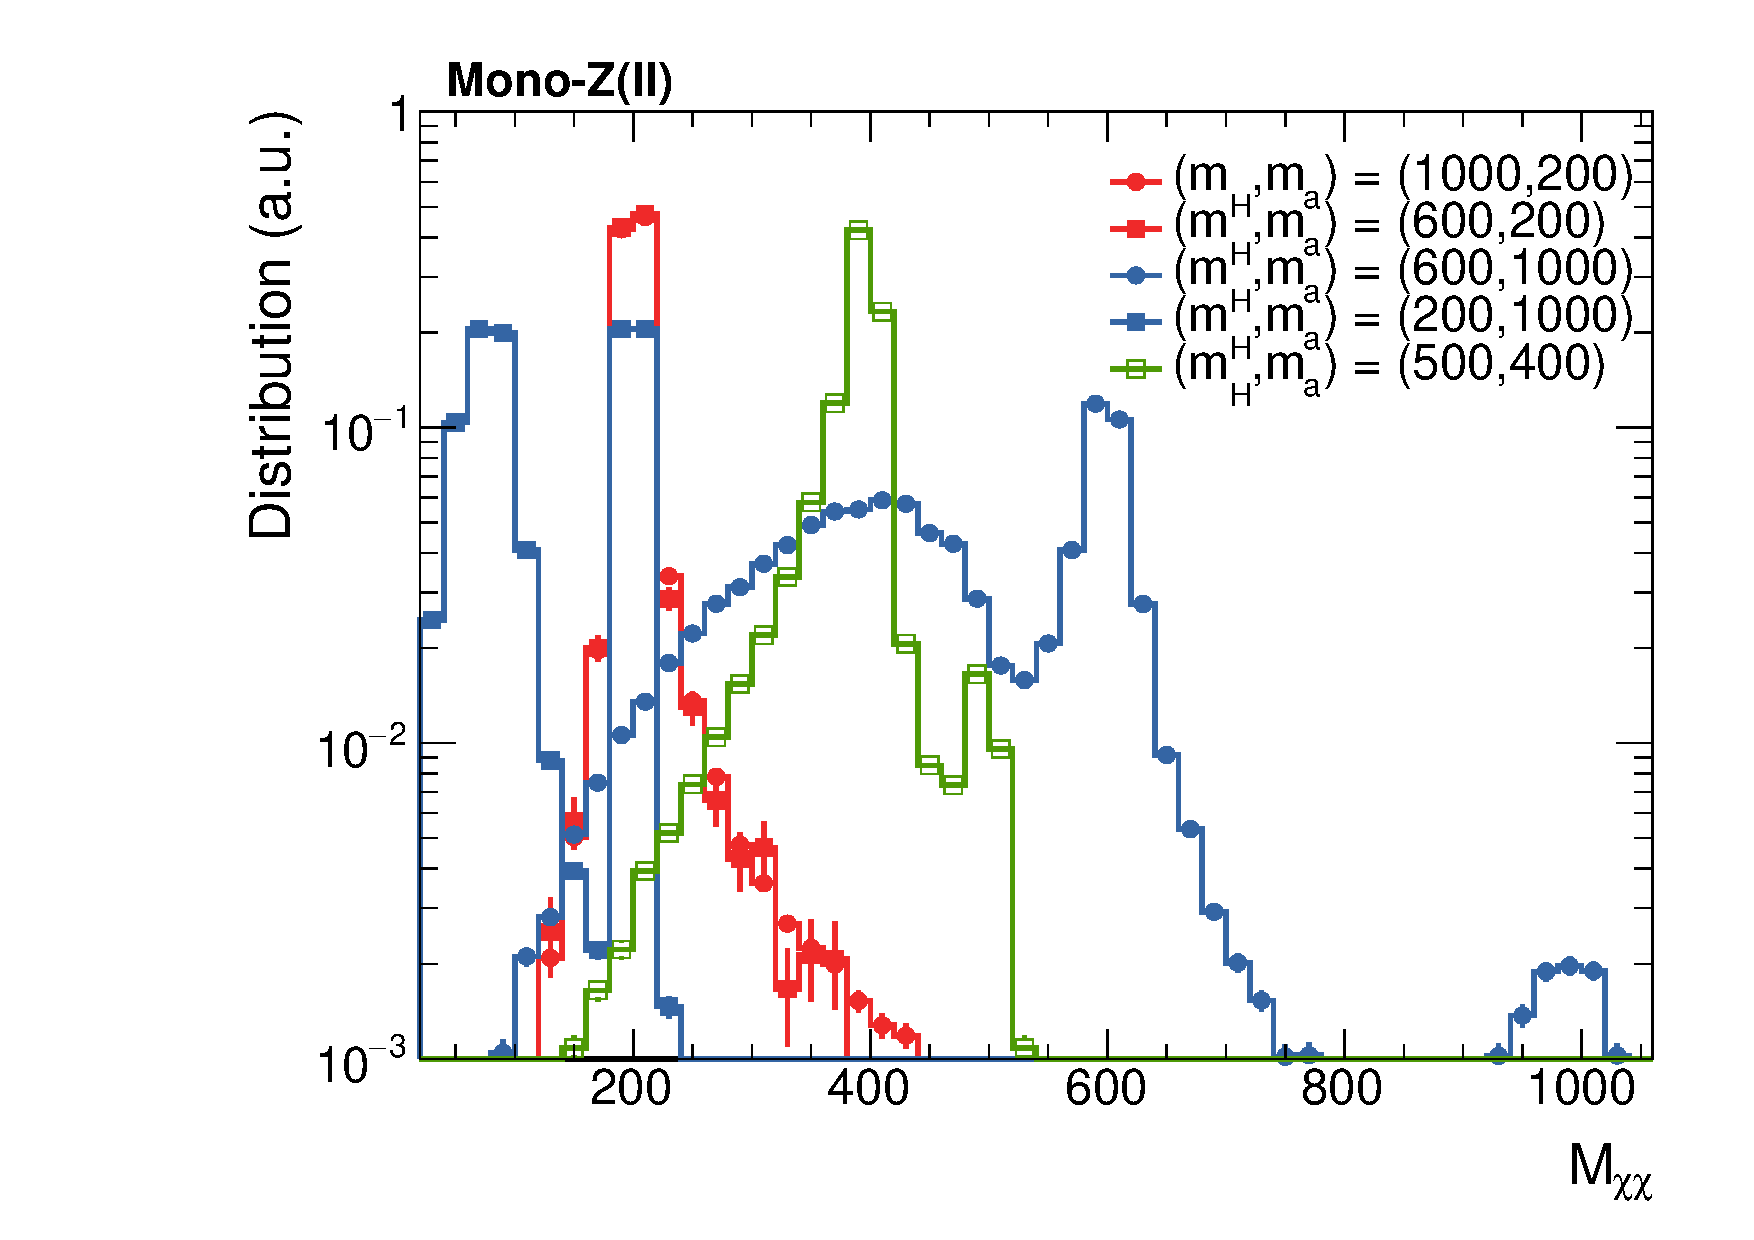
\includegraphics[width=0.45\textwidth]{texinputs/04_grid/figures/monoz/leptonic/inclusive_h_m_med_dm.pdf}
\caption{Distributions of the invariant mass of the dilepton (left) and $\chi\overline{\chi}$ systems (right) with no selection applied in addition to the generation cuts. The $M_{ll}$ distribution is centered around the Z boson mass independent of the chosen parameter point, indicating that there is no contribtion from $\gamma*$ exchange. The $M_{\chi\overline{\chi}}$ distribution }
\label{fig:monoz_kin_inclusive}
\end{figure}

The distributions of some relevant variables for this search are shown in \autoref{fig:monoz_kin_presel}, after preselection. 

\begin{figure}
\centering
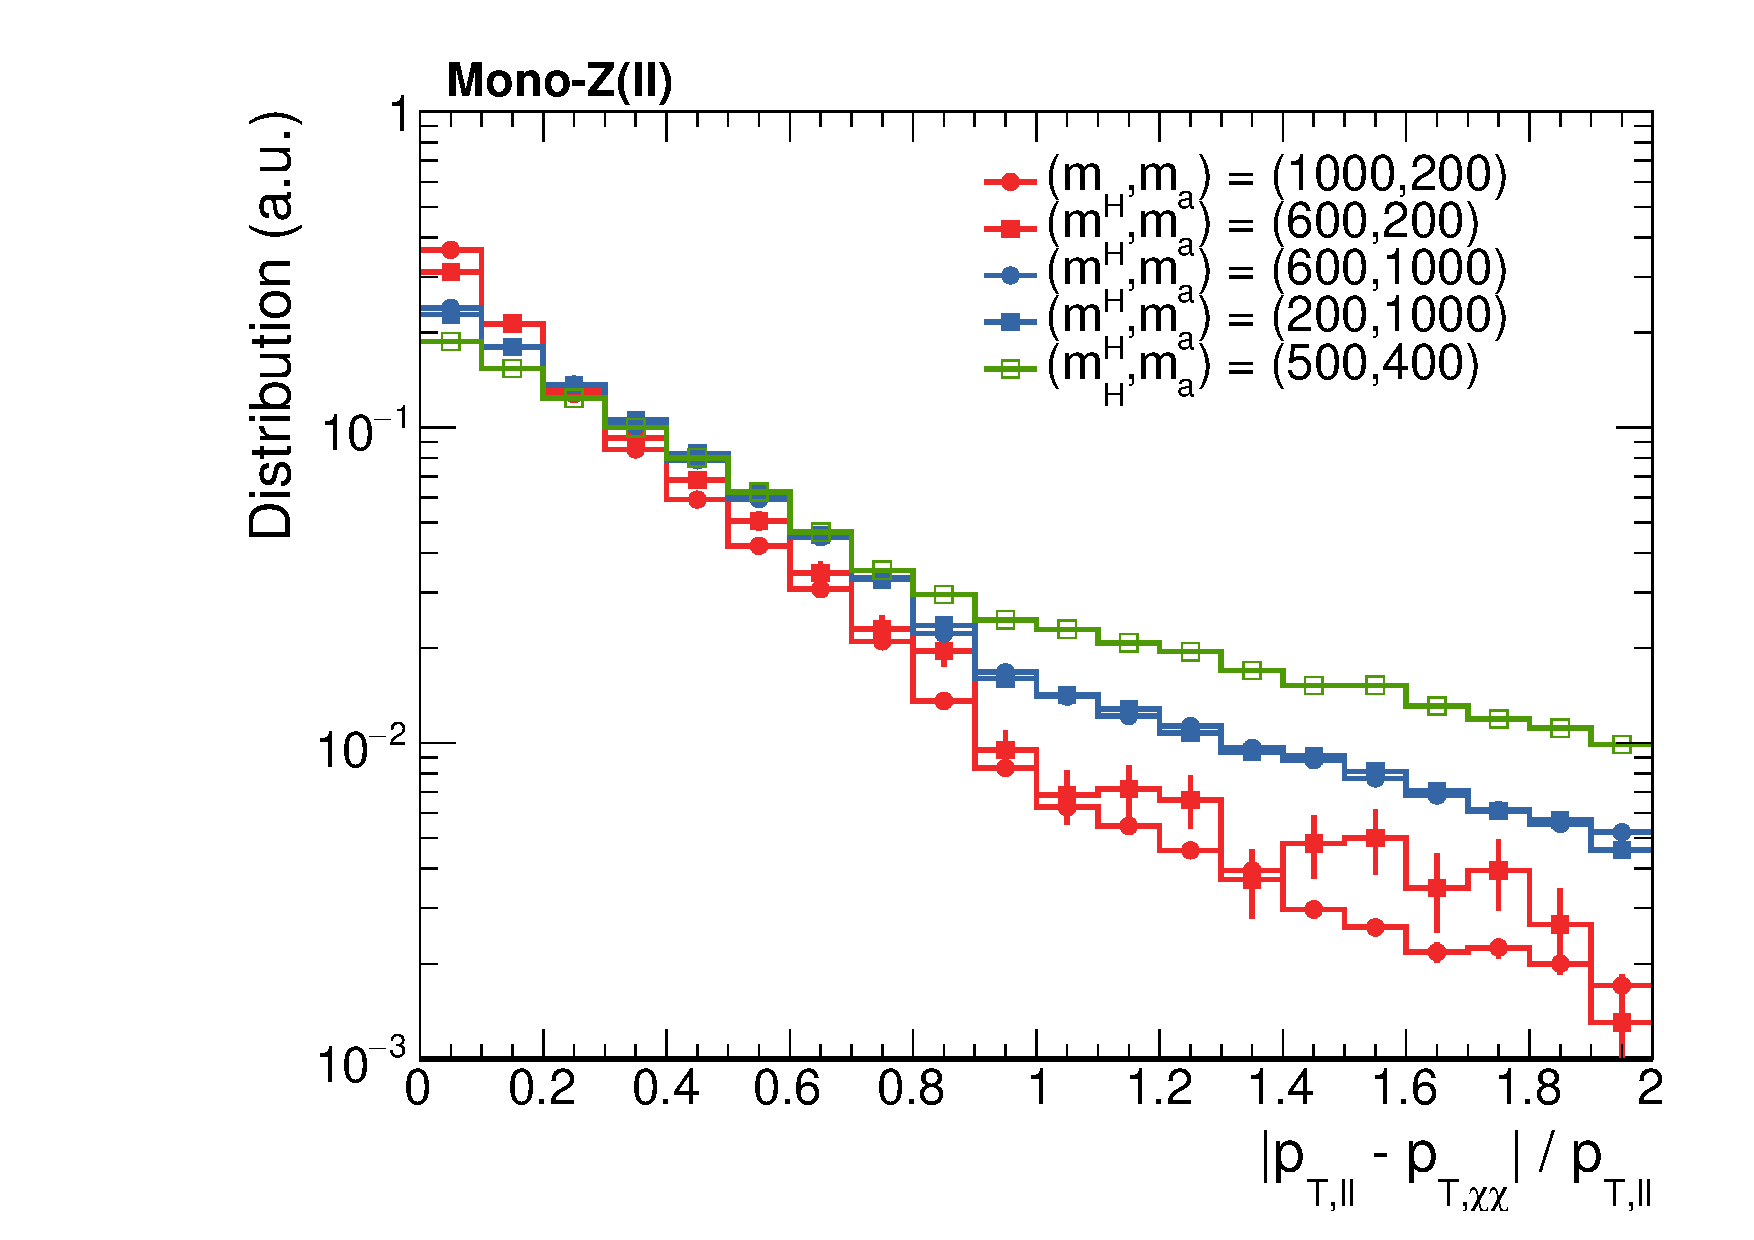
\includegraphics[width=0.45\textwidth]{texinputs/04_grid/figures/monoz/leptonic/presel_h_balance.pdf}
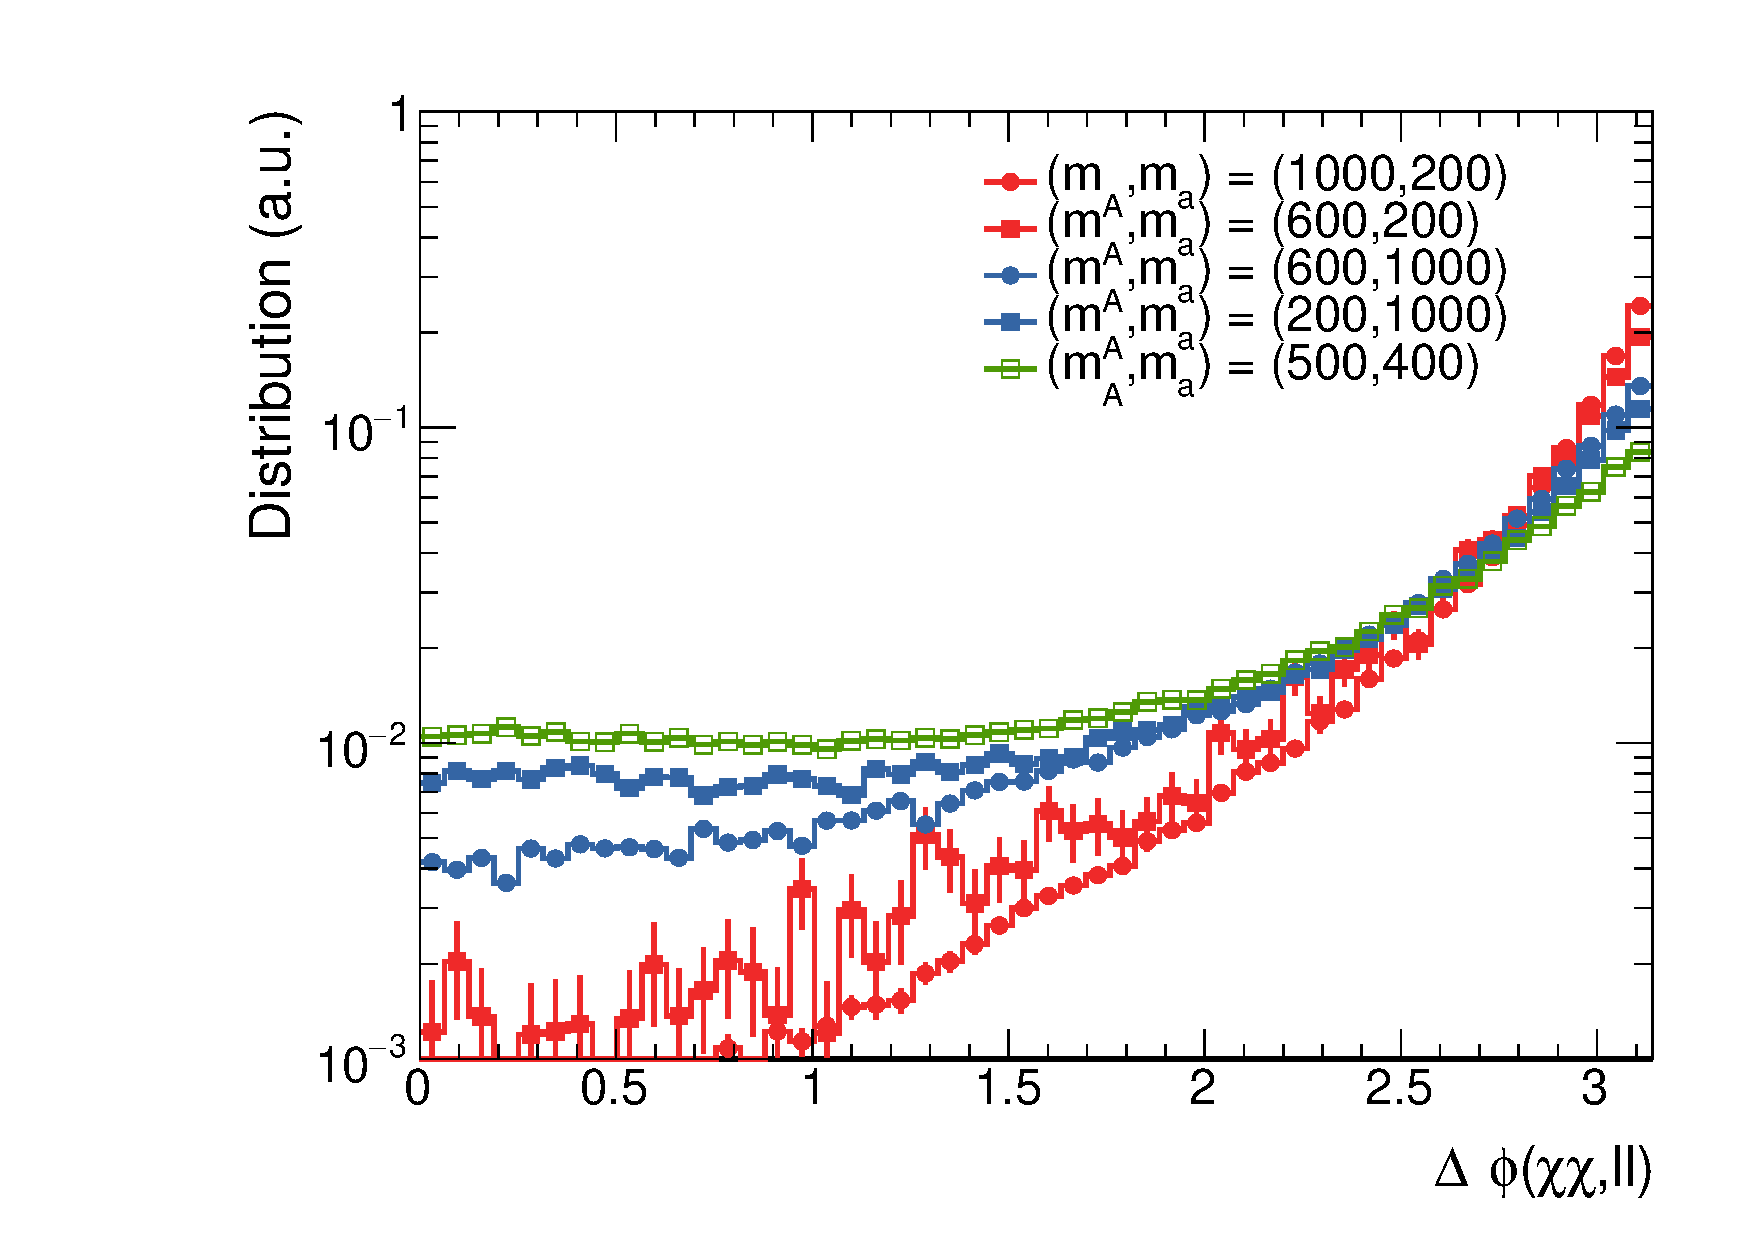
\includegraphics[width=0.45\textwidth]{texinputs/04_grid/figures/monoz/leptonic/presel_h_dphi_met_ll.pdf}
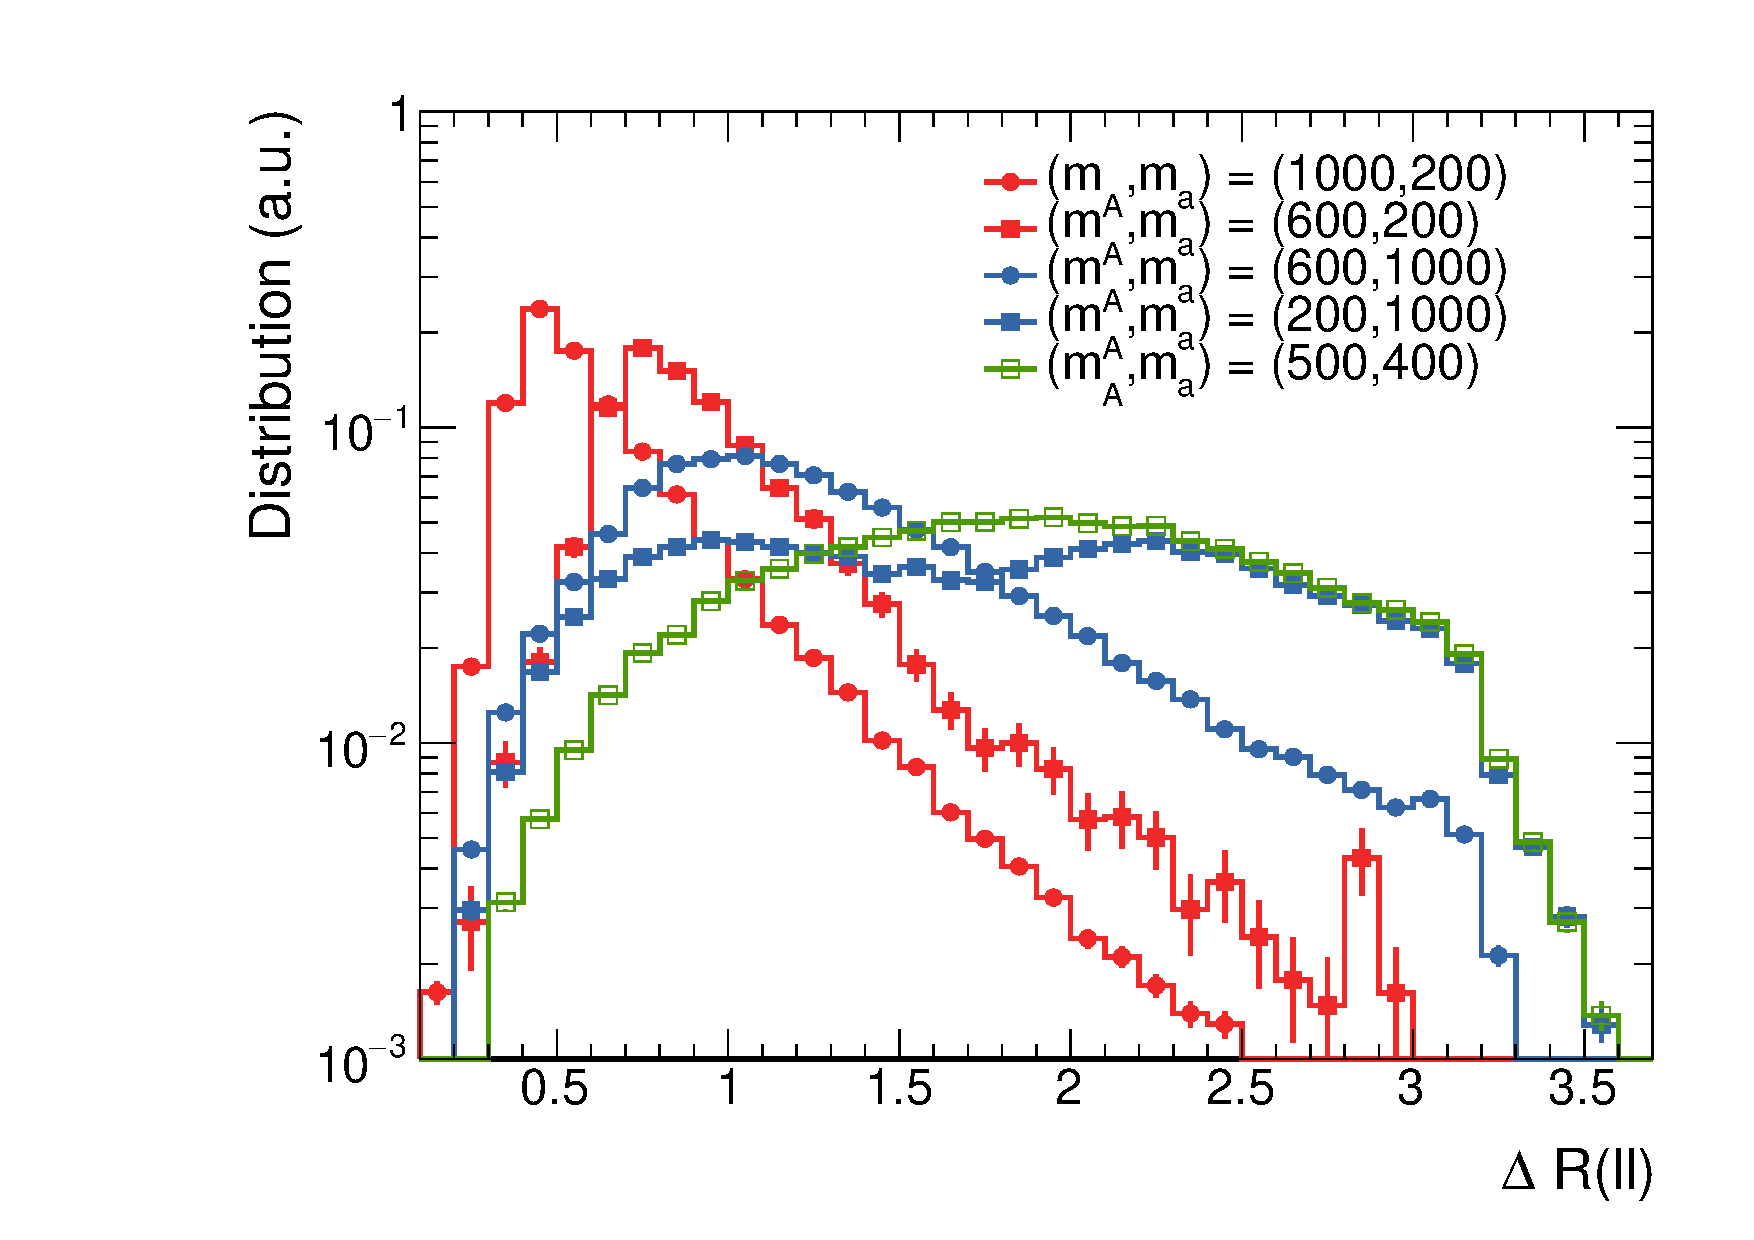
\includegraphics[width=0.45\textwidth]{texinputs/04_grid/figures/monoz/leptonic/presel_h_dr_ll.pdf}
\caption{Distributions of the main selection variables after preselection: \pt balance (top panel), $\Delta\Phi$ (middle) and $\Delta R$ (bottom). The shown parameter points illustrate the different qualitative behavior in the three different mass regions. }
\label{fig:monoz_kin_presel}
\end{figure}

\subparagraph{Z+\MET signature, hadronic channel}

The event selection criteria used in this analysis are listed in Table~\ref{tab:monozqq_selection}.

\begin{table}
\centering
\caption{Event selections used in the analysis for the mono-$Z$ hadronic signature with $Z \to q\bar{q}$ decays.
        The requirements are inspired from those used in a typical experimental analysis. 
        The $j$ ($J$) stands for the small-radius (large-radius) jet in the resolved (boosted) analysis.}
\begin{tabular}{c|c|r}
Selection stage & Quantity & Requirement \\\hline

\multirow{ 4}{*}{Inclusive resolved and boosted selections}  & Jet radius & $=0.4$ (1.0)\\
                                          & Jet $\left|\eta\right|$  & $<2.5$ (2.0)\\
                                          & Jet \pt                       & $>25$ GeV (200)\\
                                          & Number of jets         & $\geq2$ (1)\\\hline
\multirow{ 3}{*}{Final resolved and boosted selections}   & $|m_{jj {\,\text{or}\,} J} - m_Z|$             & $<15$ GeV\\
                                                    & $\Delta\Phi(jj {\,\text{or}\,} J, \MET)$    & $>2$\\
                                                    &  $\MET$                             & $>100$ (250) GeV\\
\end{tabular}
\label{tab:monozqq_selection}
\end{table}

Figure~\ref{fig:monozhad_kin_inc_fixed_ma} shows the kinematic distributions of mono-$Z$ events after applying 
the inclusive selections, separately for the resolved and boosted topologies. The \ma is fixed to 250~GeV and the \mA is
chosen to be 300, 600, 900 and 1200~GeV in the figure. When the \mA gets closer to \ma, the $Z$-boson
is less boosted, causing the large-radius jet mass to be more populated at mass below $\sim30$~GeV. 
When the $|\mA-\ma|$ becomes smaller than the $Z$-boson mass, the non-resonant production dominates as clearly
seen in the \MET spectrum for the resolved case.
Figure~\ref{fig:monozhad_kin_inc_fixed_mA} shows the same set of distributions when the \mA is fixed to 600~GeV 
and the \ma varies from 150 to 250, 350 and 450~GeV. 
The trend seen in Fig.~\ref{fig:monozhad_kin_inc_fixed_ma} is also visible here when the \ma gets closer to \mA.


\begin{figure}
\centering
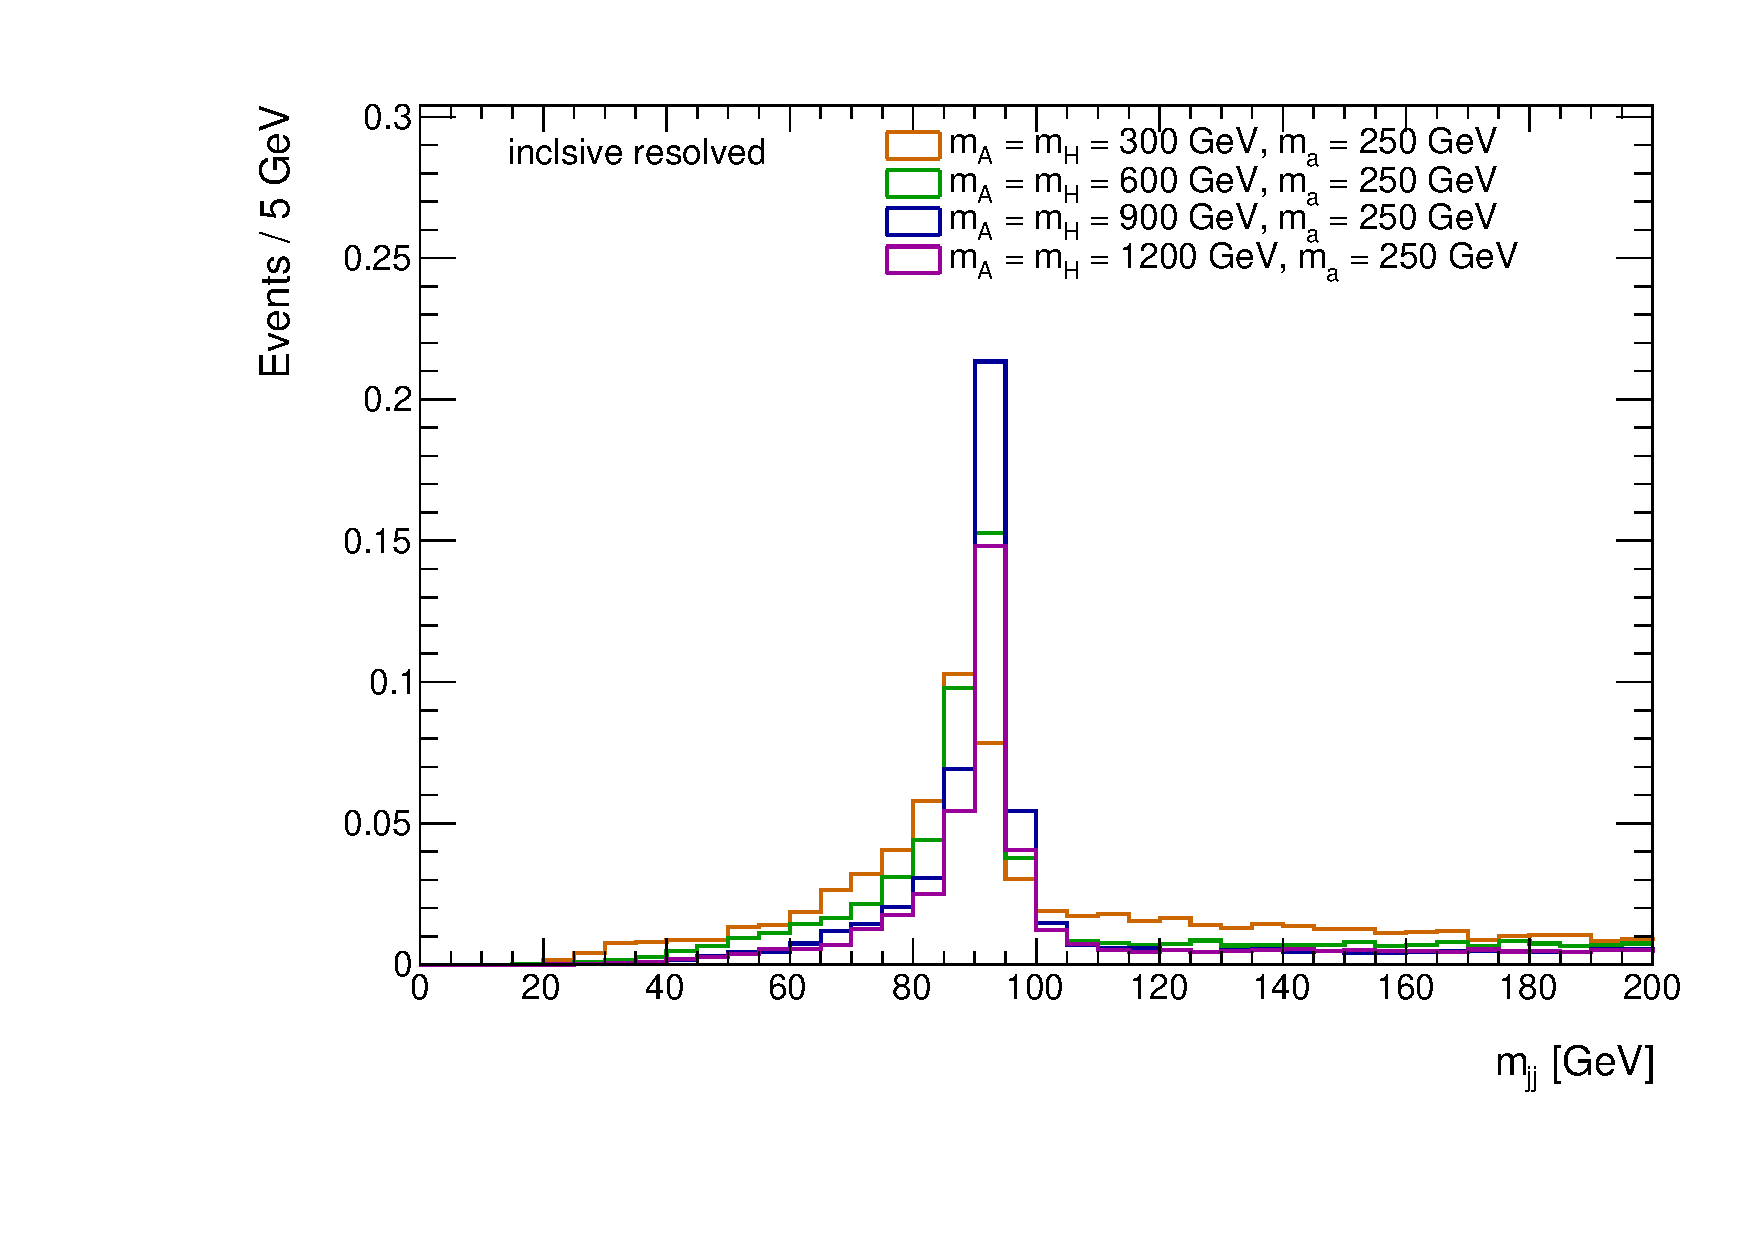
\includegraphics[width=0.45\textwidth]{texinputs/04_grid/figures/monoz/hadronic/ma250_incl_resl_MJJ_linear.pdf}
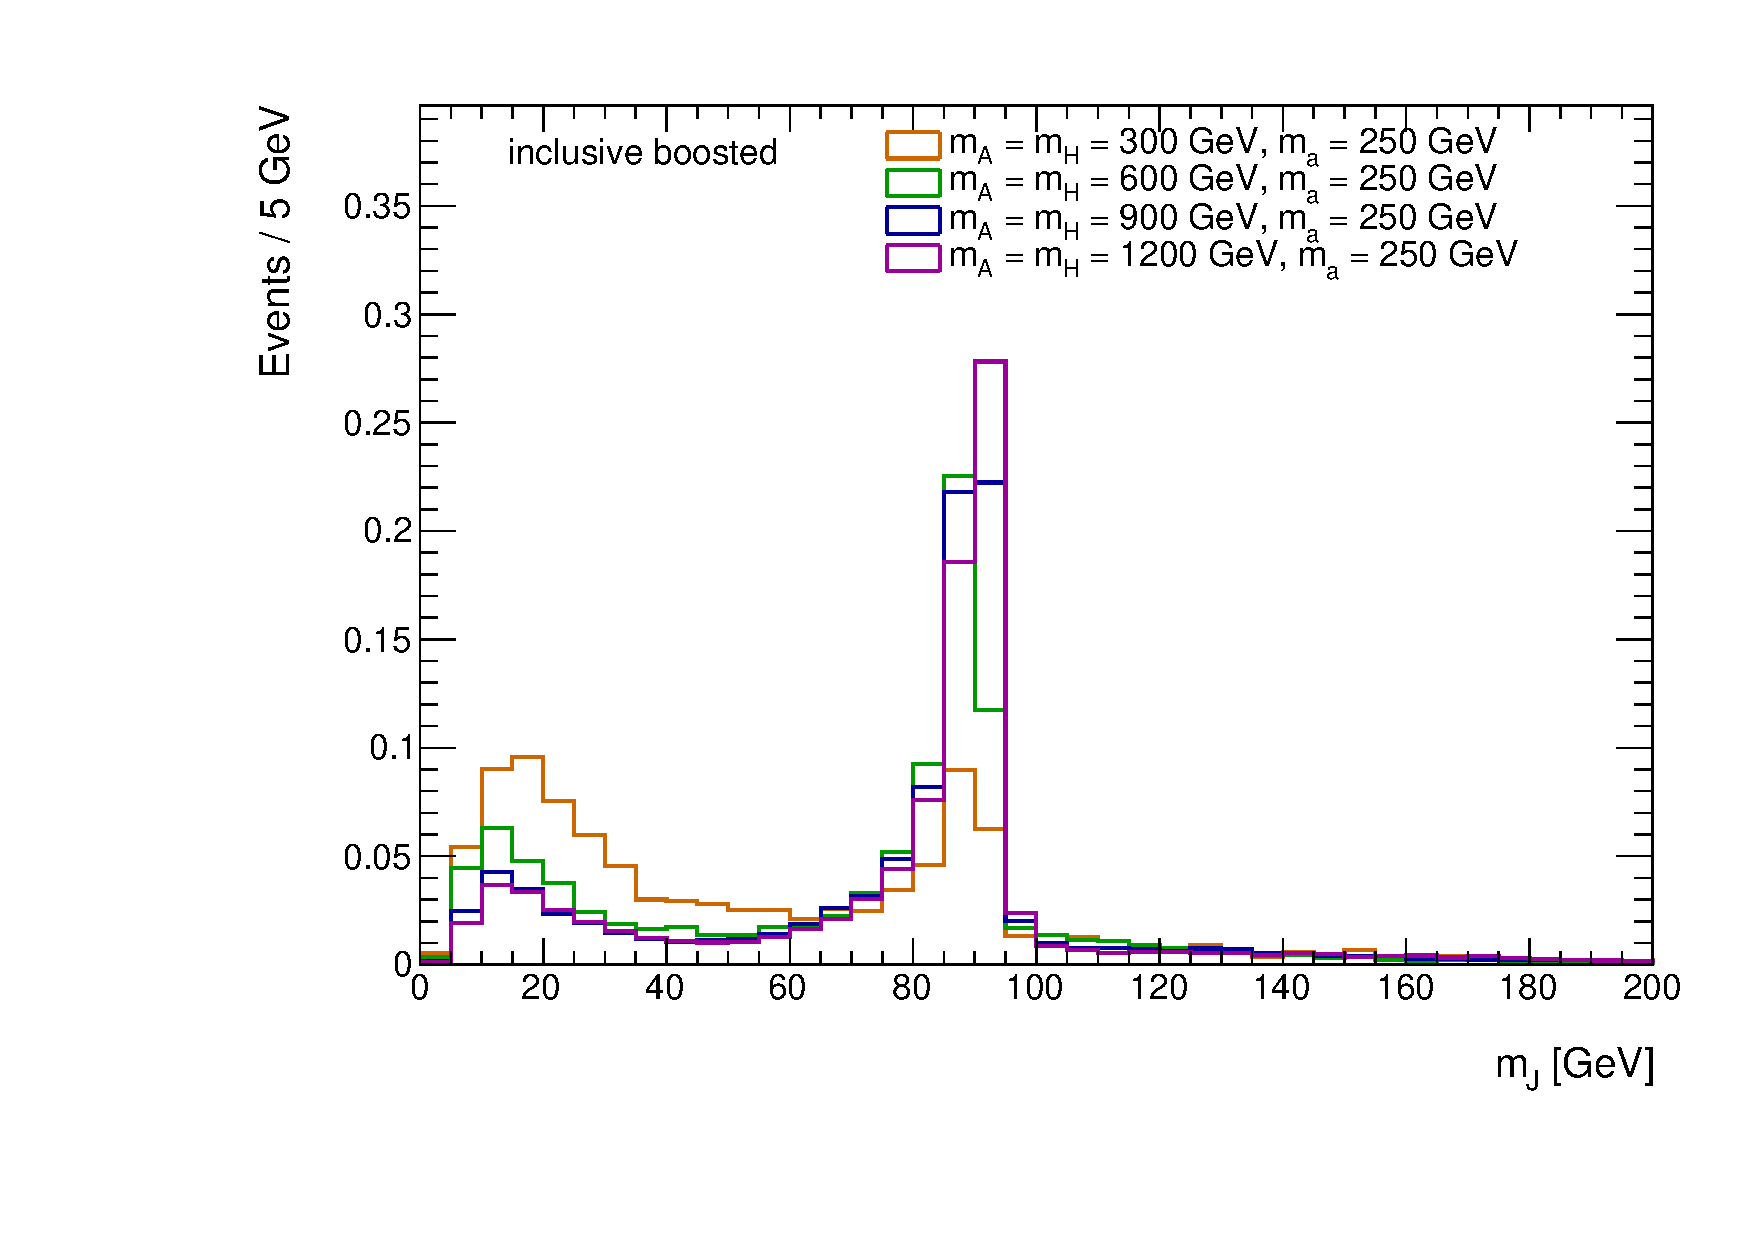
\includegraphics[width=0.45\textwidth]{texinputs/04_grid/figures/monoz/hadronic/ma250_incl_merged_MFatJ1_linear.pdf}
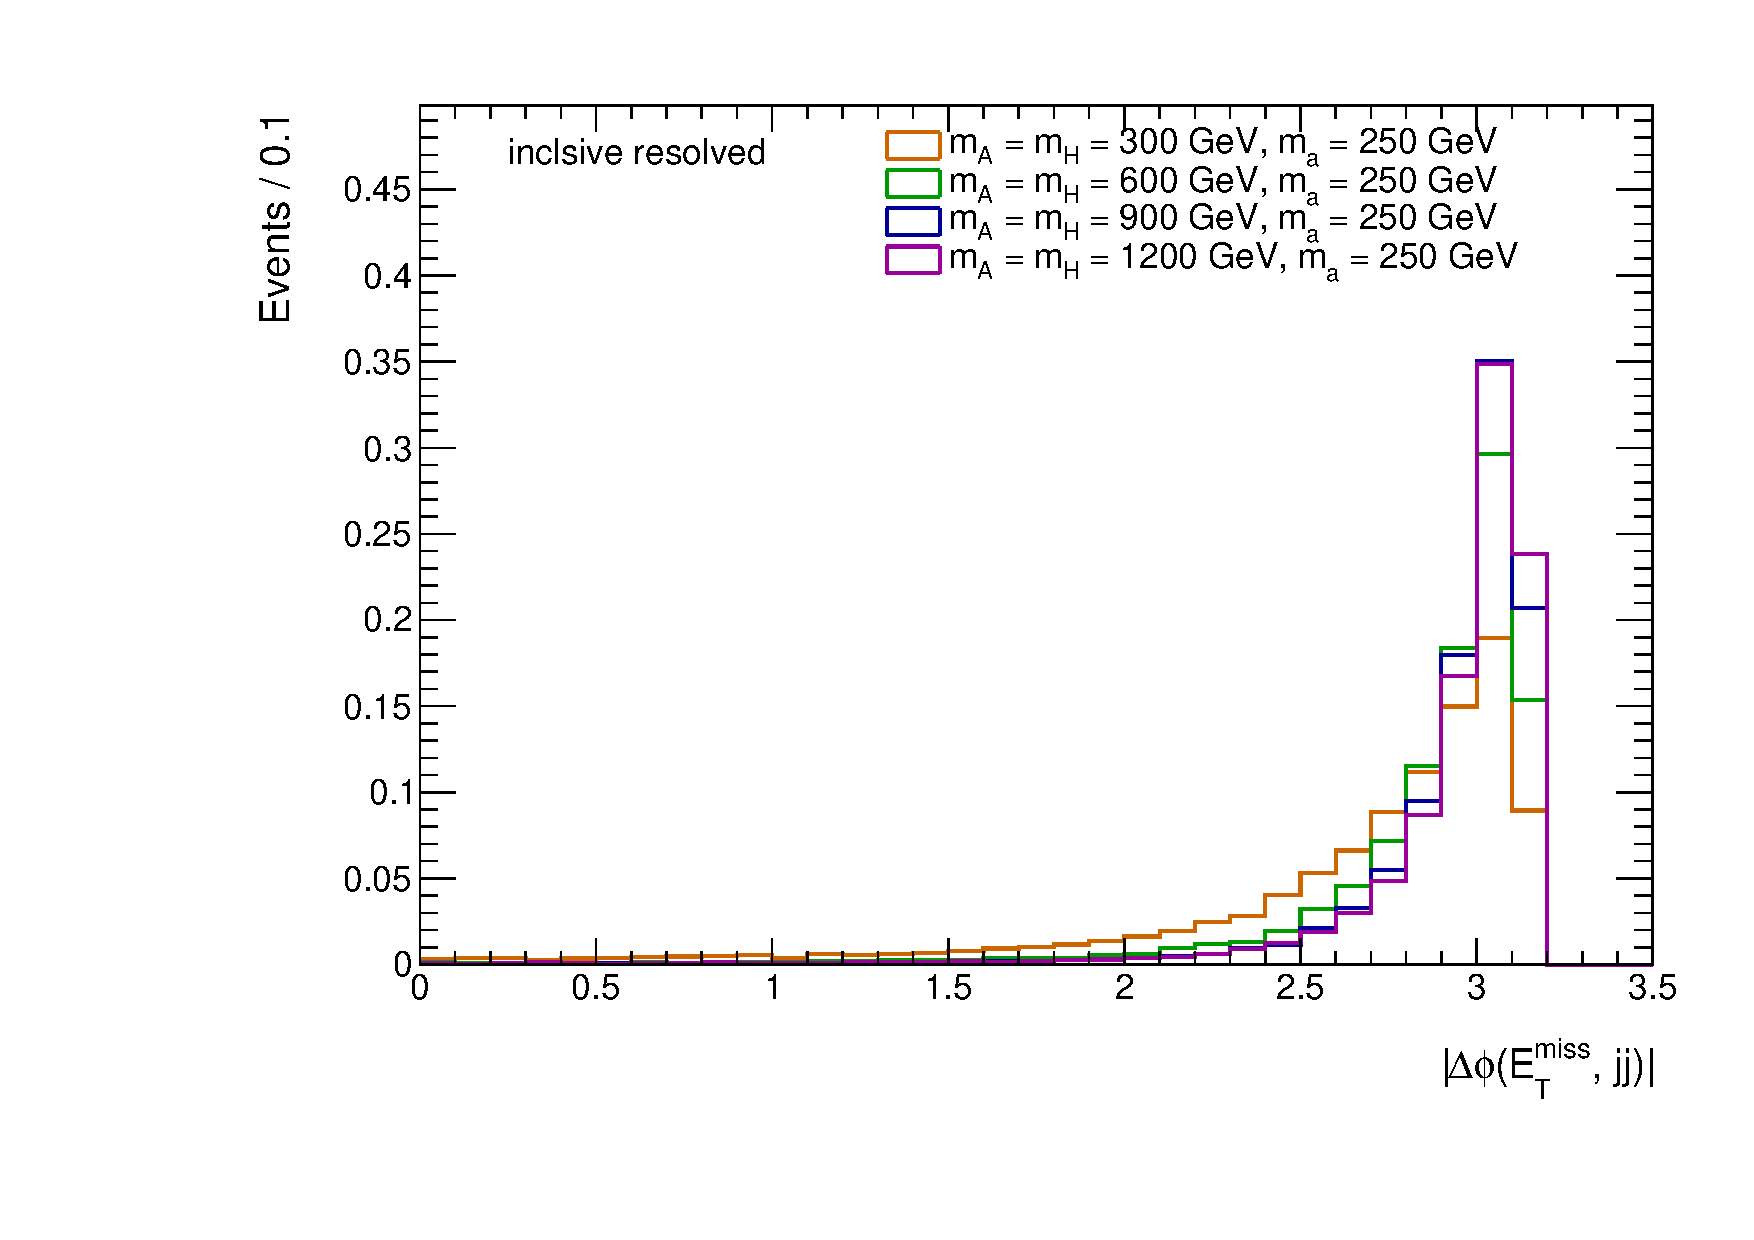
\includegraphics[width=0.45\textwidth]{texinputs/04_grid/figures/monoz/hadronic/ma250_incl_resl_dPhiMETJJ_linear.pdf}
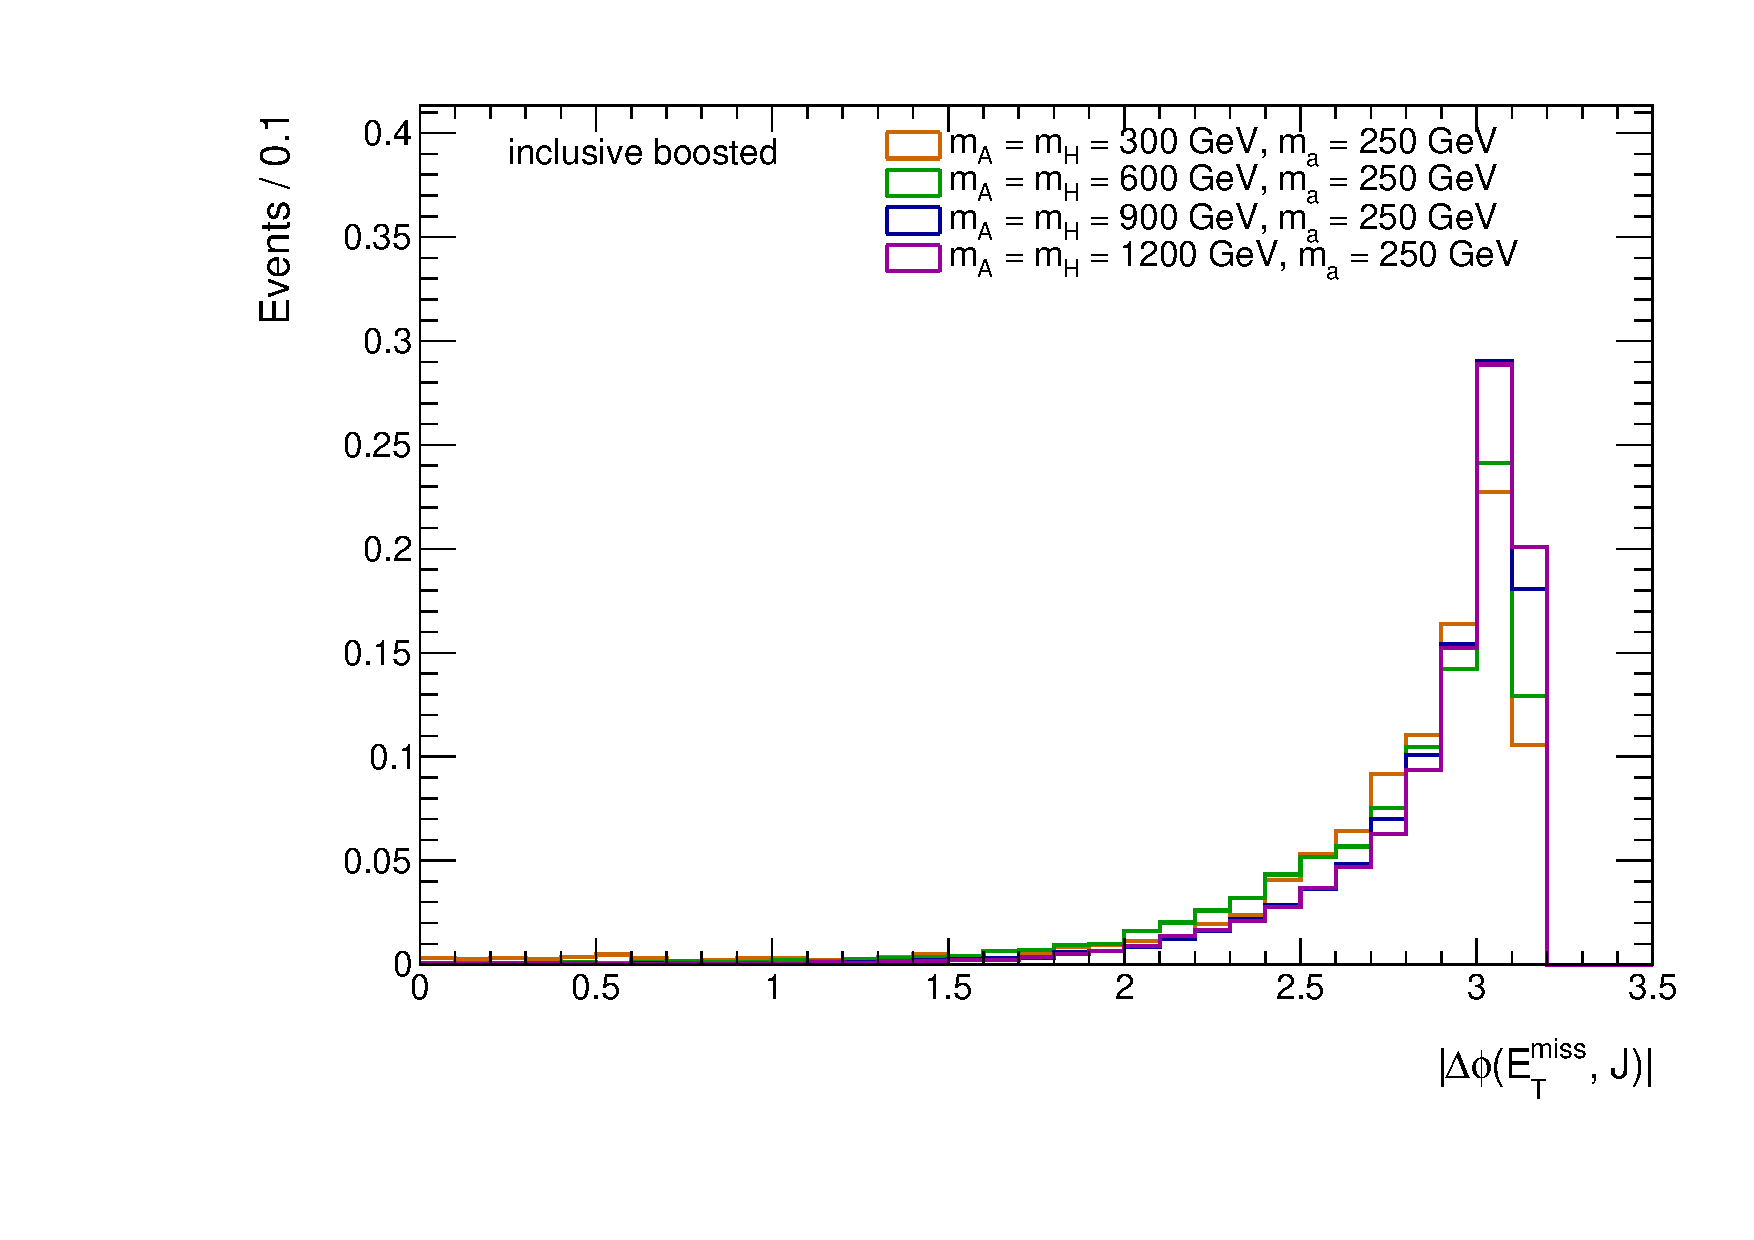
\includegraphics[width=0.45\textwidth]{texinputs/04_grid/figures/monoz/hadronic/ma250_incl_merged_dPhiMETJ_linear.pdf}
\caption{Dijet mass (top), $\Delta\Phi(jj, \MET)$ (bottom) distributions 
after applying the inclusive selections in the resolved analysis are shown on the left side. Large-radius 
jet mass (top), $\Delta\Phi(J, \MET)$ (bottom) distributions 
after applying the inclusive selections in the boosted analysis are shown on the right side. 
The signal masses are chosen to be \mA = 300, 600, 900 and 1200~GeV with the fixed \ma = 250~GeV.}
\label{fig:monozhad_kin_inc_fixed_ma}
\end{figure}

\begin{figure}
\centering
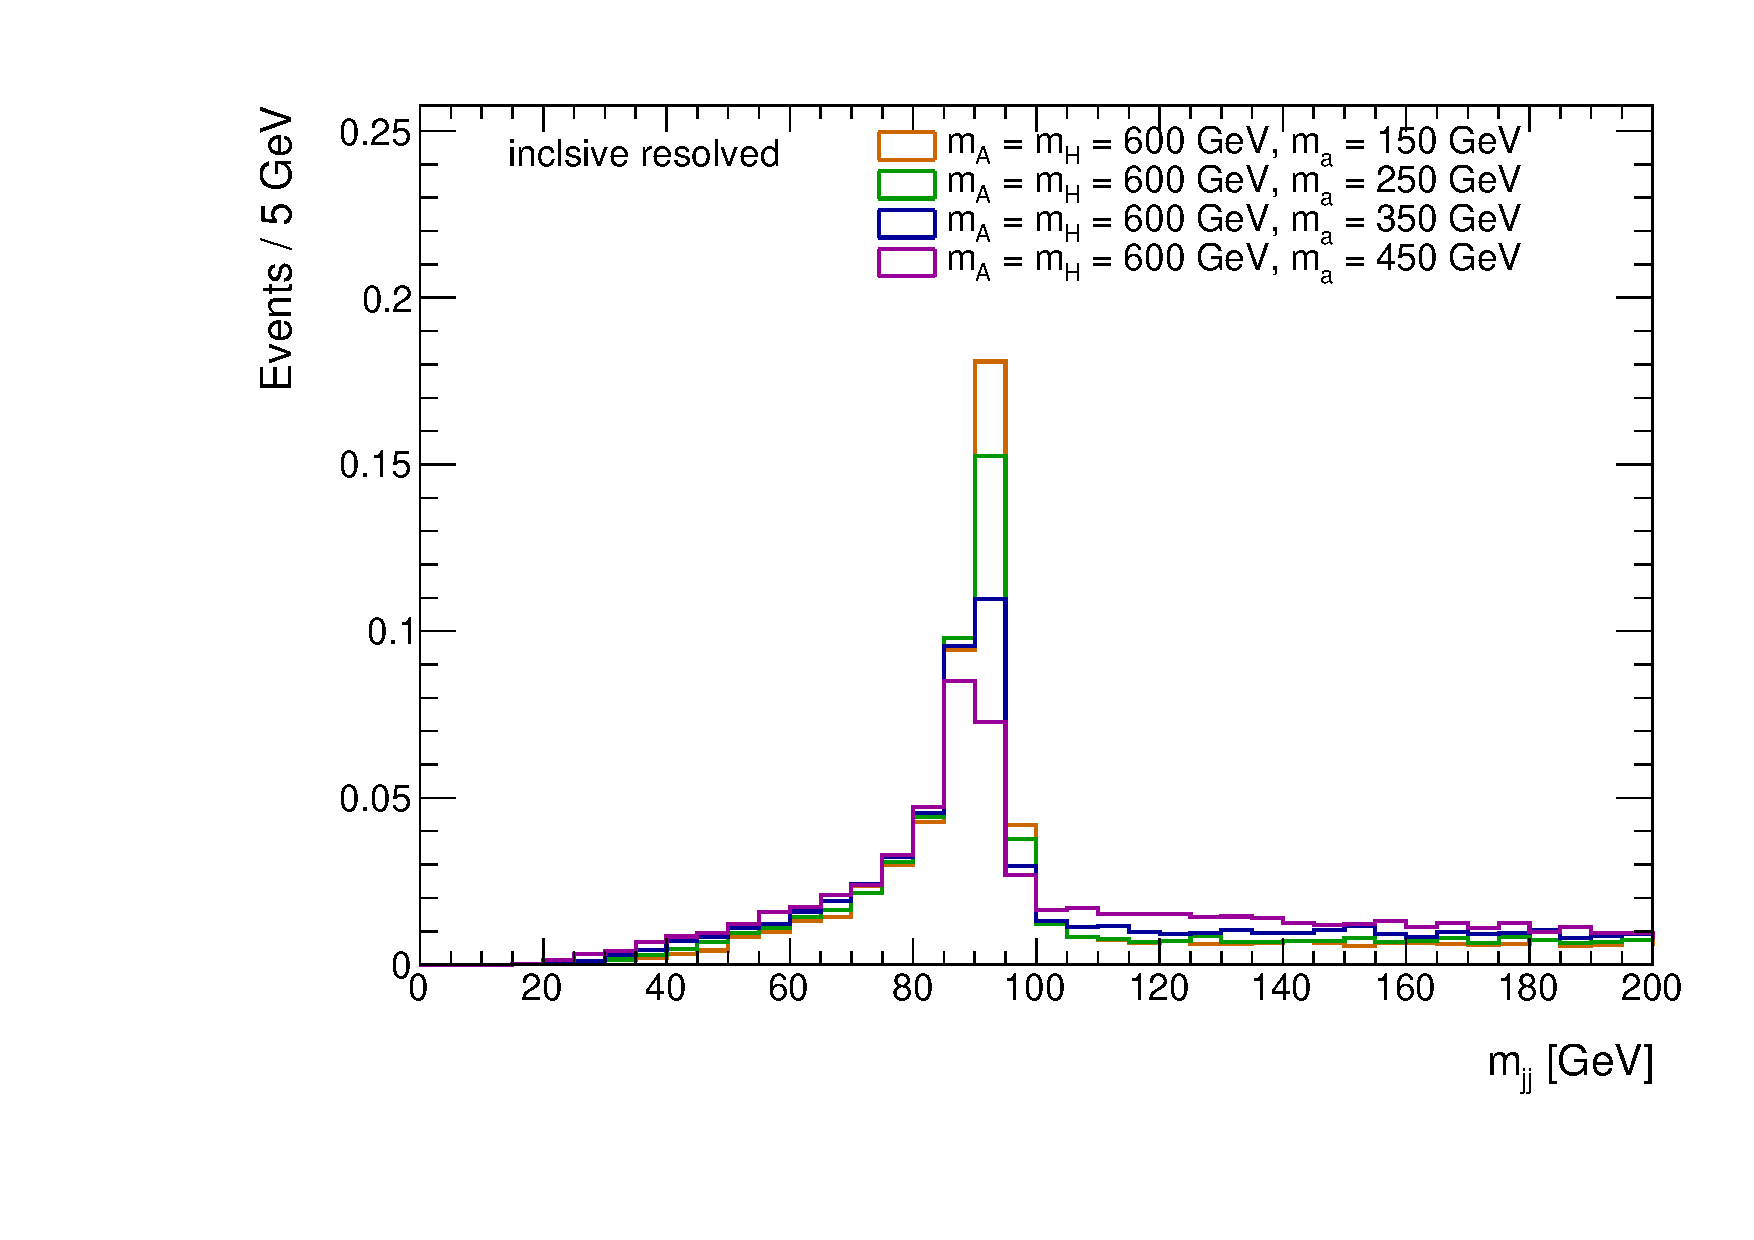
\includegraphics[width=0.45\textwidth]{texinputs/04_grid/figures/monoz/hadronic/mA600_incl_resl_MJJ_linear.pdf}
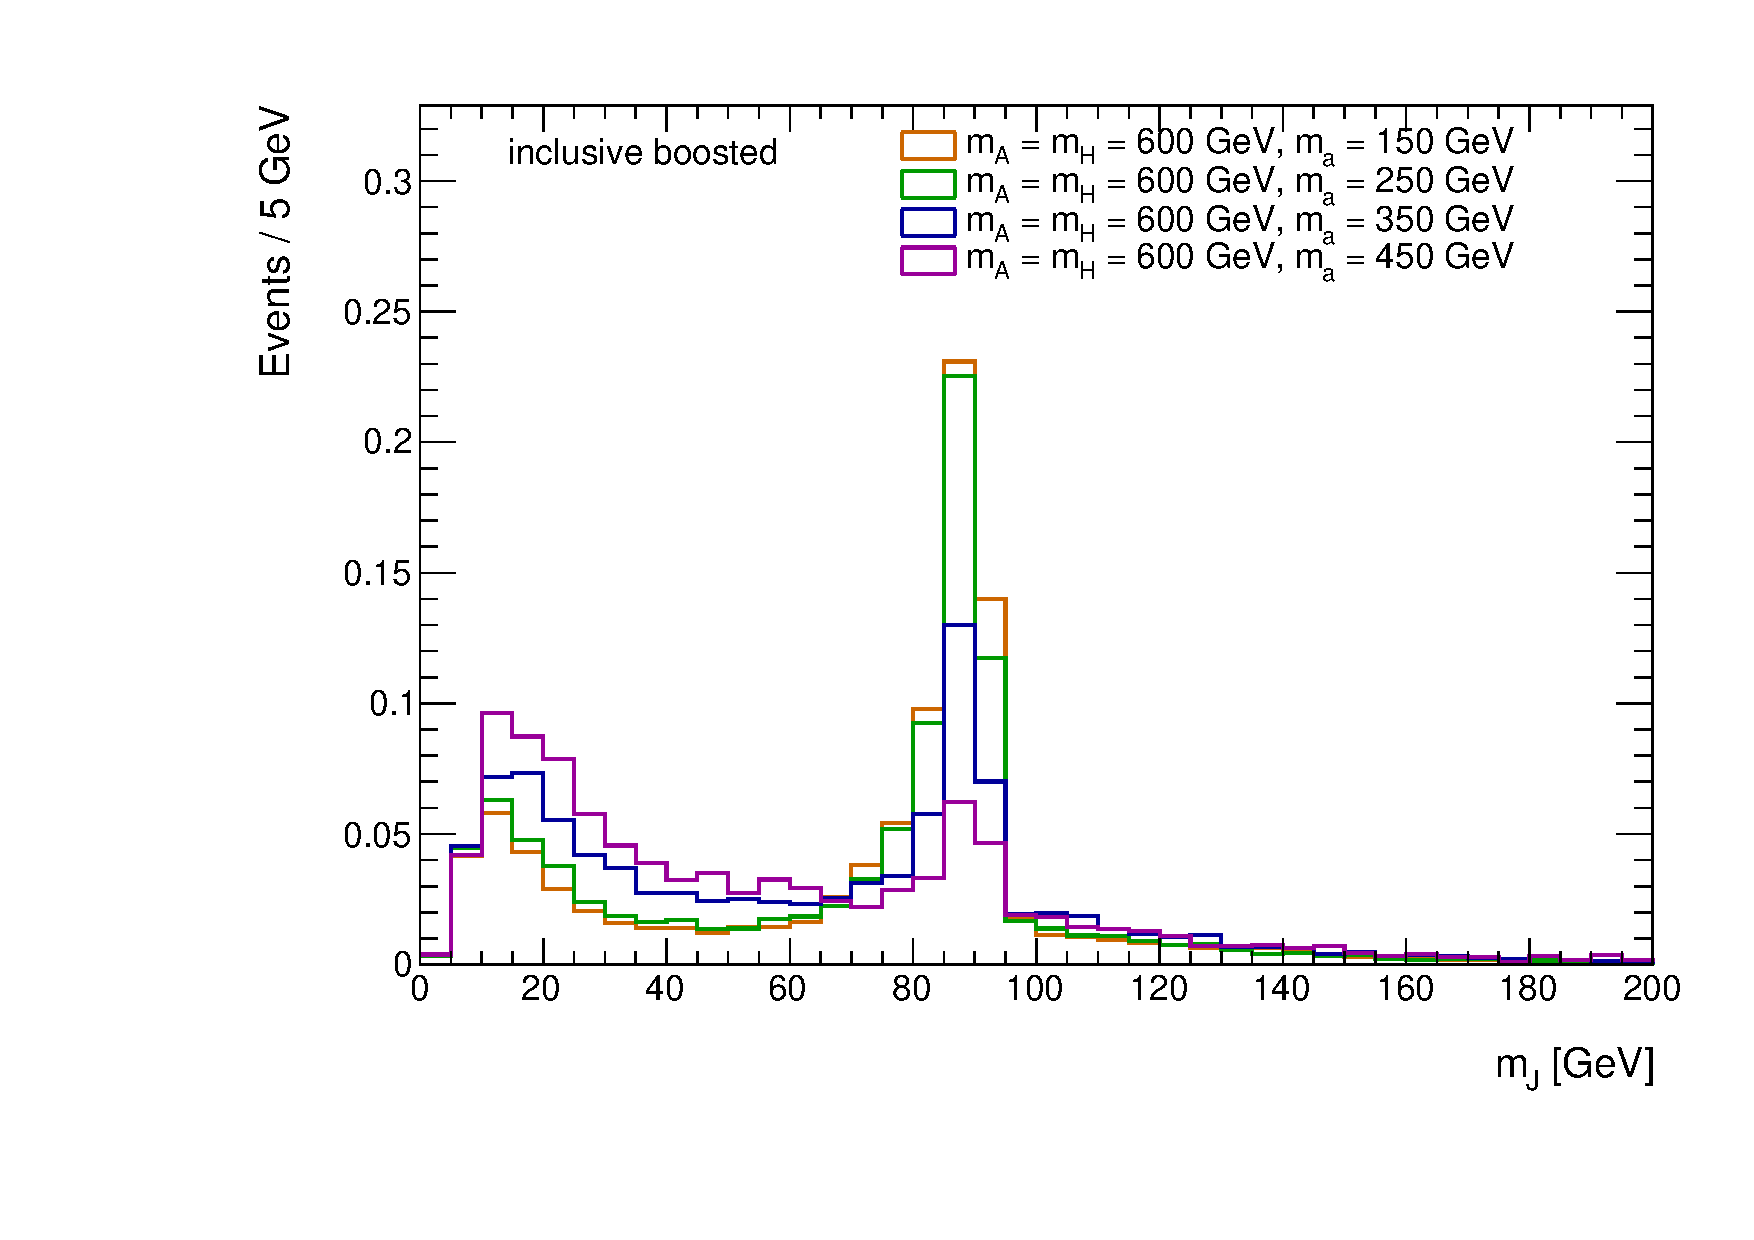
\includegraphics[width=0.45\textwidth]{texinputs/04_grid/figures/monoz/hadronic/mA600_incl_merged_MFatJ1_linear.pdf}
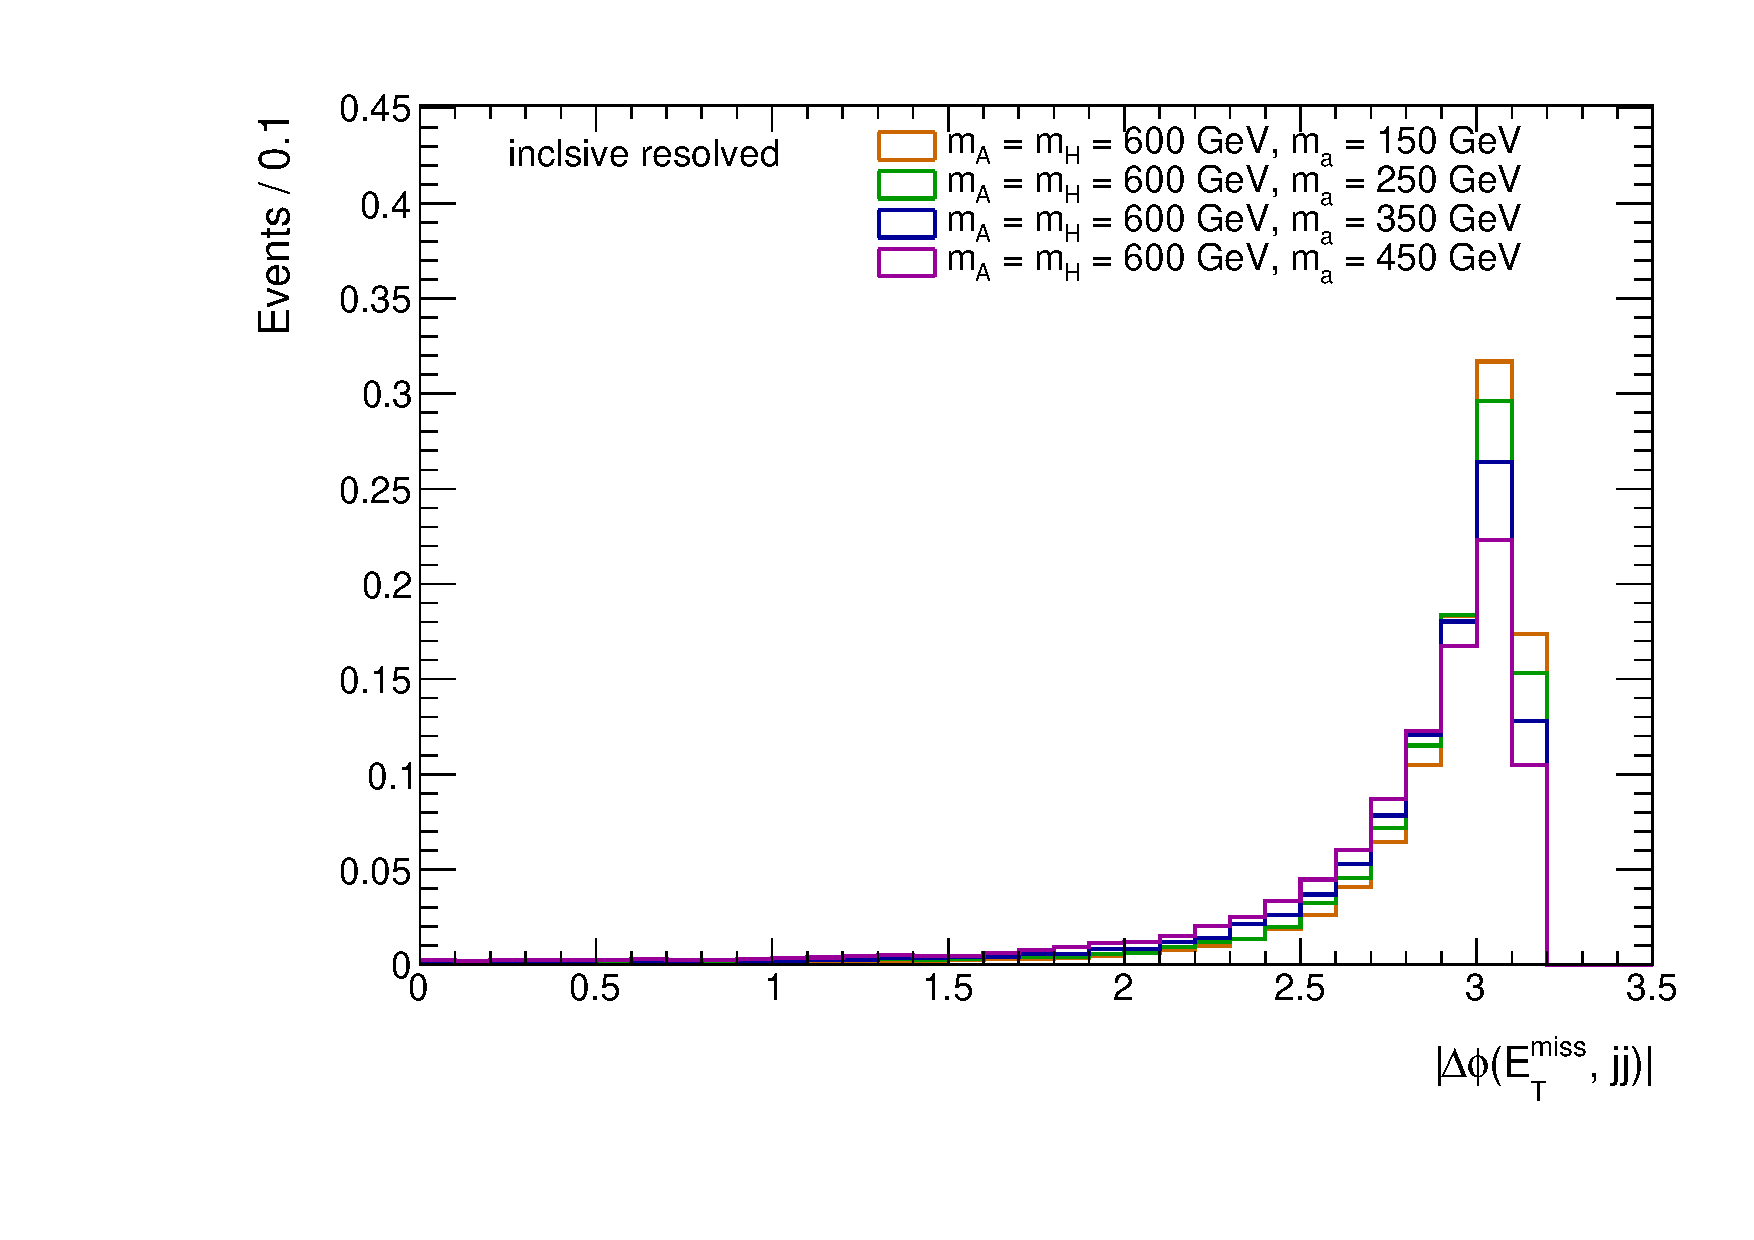
\includegraphics[width=0.45\textwidth]{texinputs/04_grid/figures/monoz/hadronic/mA600_incl_resl_dPhiMETJJ_linear.pdf}
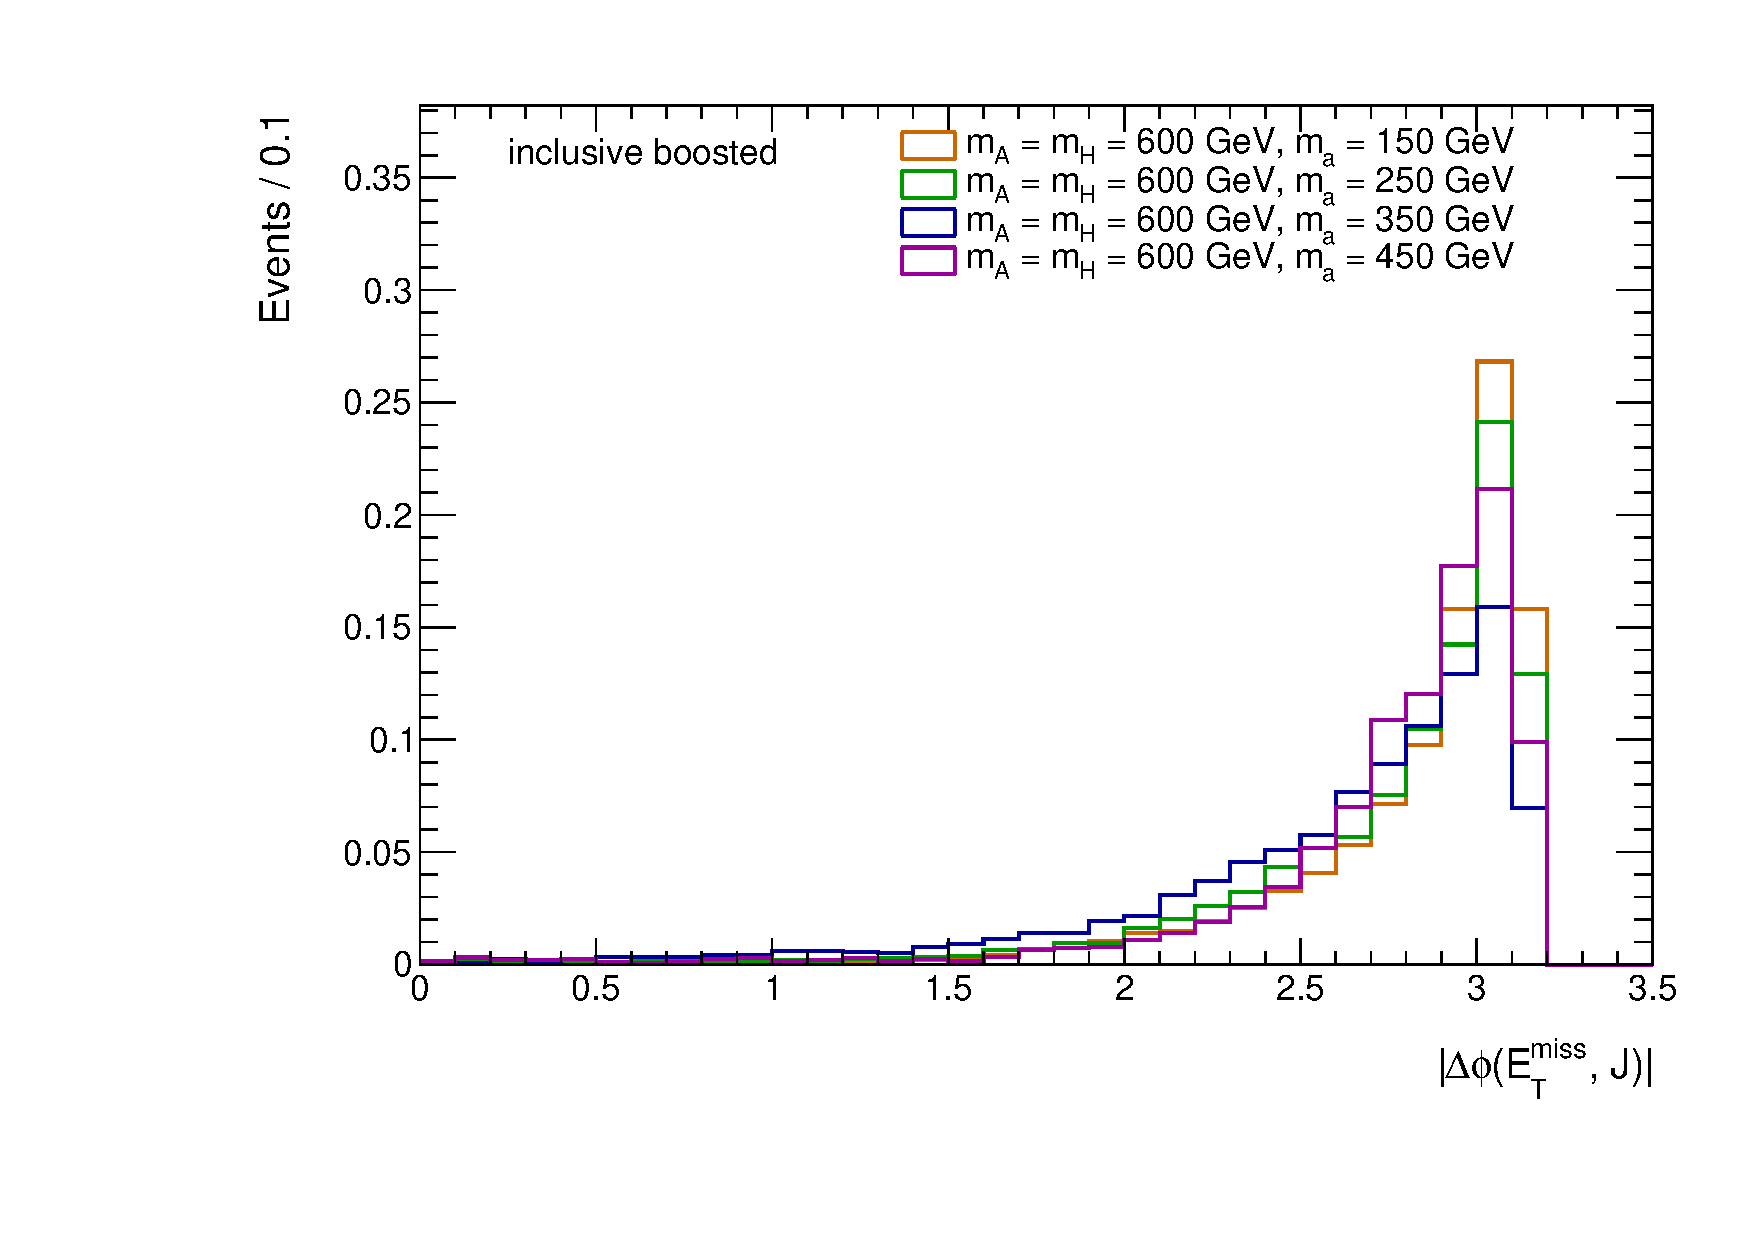
\includegraphics[width=0.45\textwidth]{texinputs/04_grid/figures/monoz/hadronic/mA600_incl_merged_dPhiMETJ_linear.pdf}
\caption{Dijet mass (top), $\Delta\Phi(jj, \MET)$ (bottom) distributions 
after applying the inclusive selections in the resolved analysis are shown on the left side. Large-radius 
jet mass (top), $\Delta\Phi(J, \MET)$ (bottom) distributions 
after applying the inclusive selections in the boosted analysis are shown on the right side. 
The signal masses are chosen to be \ma = 150, 250, 350 and 450~GeV with the fixed \mA = 600~GeV.}
\label{fig:monozhad_kin_inc_fixed_mA}
\end{figure}



